\documentclass[tikz,border=0pt]{standalone}
\usepackage[utf8]{inputenc}
\usepackage[T1]{fontenc}
\usepackage{lmodern}
\usepackage{amsmath,amssymb}
\usetikzlibrary{arrows.meta,positioning,fit,calc,backgrounds,shapes.geometric,decorations.pathreplacing}
\definecolor{navy}{HTML}{163A5F}
\definecolor{blue}{HTML}{2C6EAF}
\definecolor{lightblue}{HTML}{EAF2F8}
\definecolor{midblue}{HTML}{CFE1F2}
\definecolor{graytext}{HTML}{4A5560}
\definecolor{lightgray}{HTML}{F4F6F8}
\definecolor{green}{HTML}{3C8D73}
\definecolor{lightgreen}{HTML}{E8F5EF}
\definecolor{red}{HTML}{B24A4A}
\definecolor{lightred}{HTML}{FBEDEE}
\tikzset{
  title/.style={font=\sffamily\bfseries\fontsize{16}{18}\selectfont,text=navy,anchor=west},
  subtitle/.style={font=\sffamily\bfseries\fontsize{11}{13}\selectfont,text=navy},
  body/.style={font=\sffamily\fontsize{9.2}{11}\selectfont,text=graytext,align=left},
  small/.style={font=\sffamily\fontsize{8}{9.4}\selectfont,text=graytext,align=left},
  tinylabel/.style={font=\sffamily\fontsize{7.2}{8.4}\selectfont,text=graytext},
  panel/.style={rounded corners=3pt,draw=midblue,fill=white,line width=0.6pt},
  box/.style={rounded corners=2pt,draw=midblue,fill=lightblue,line width=0.6pt},
  worker/.style={rounded corners=2pt,draw=blue,dashed,line width=0.7pt,fill=white},
  task/.style={rounded corners=2pt,draw=blue,fill=lightblue,minimum width=0.85cm,minimum height=0.55cm,font=\sffamily\bfseries\small,text=navy},
  file/.style={draw=blue,fill=white,minimum width=0.55cm,minimum height=0.42cm,font=\sffamily\small,text=navy},
  arr/.style={-{Stealth[length=2.4mm,width=1.8mm]},draw=blue,line width=0.9pt},
  arrthin/.style={-{Stealth[length=2mm,width=1.5mm]},draw=blue,line width=0.7pt},
  arrred/.style={-{Stealth[length=2mm,width=1.5mm]},draw=red,dashed,line width=0.8pt},
  arrgreen/.style={-{Stealth[length=2mm,width=1.5mm]},draw=green,dotted,line width=1pt}
}
\begin{document}

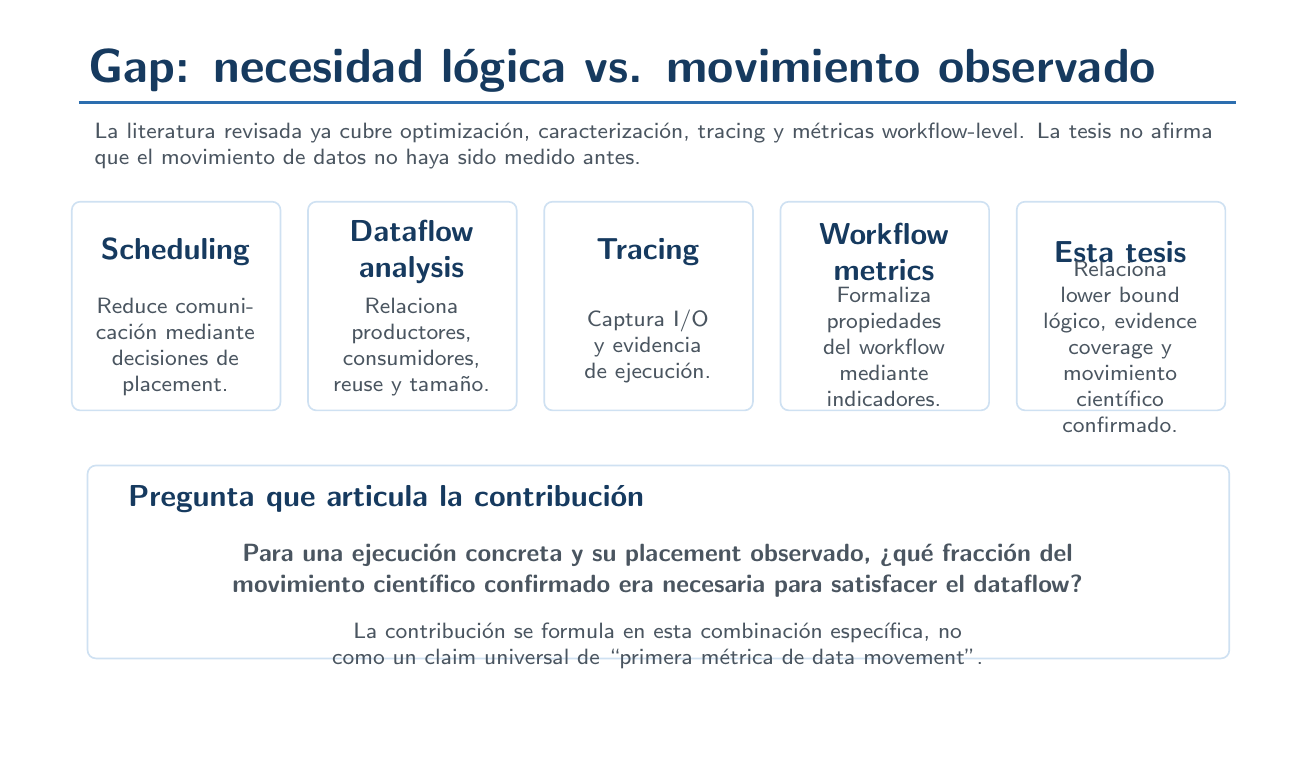
\begin{tikzpicture}[x=1cm,y=1cm]
\path[use as bounding box] (0,0) rectangle (16,9);
\node[title] at (0.65,8.45) {Gap: necesidad lógica vs. movimiento observado};
\draw[blue,line width=1pt] (0.65,8.05)--(15.35,8.05);
\node[small,text width=14.3cm] at (8,7.5) {La literatura revisada ya cubre optimización, caracterización, tracing y métricas workflow-level. La tesis no afirma que el movimiento de datos no haya sido medido antes.};
\foreach \x/\ttl/\txt in {
0.55/{Scheduling}/{Reduce comunicación mediante decisiones de placement.},
3.55/{Dataflow analysis}/{Relaciona productores, consumidores, reuse y tamaño.},
6.55/{Tracing}/{Captura I/O y evidencia de ejecución.},
9.55/{Workflow metrics}/{Formaliza propiedades del workflow mediante indicadores.},
12.55/{Esta tesis}/{Relaciona lower bound lógico, evidence coverage y movimiento científico confirmado.}}
{
\node[panel,minimum width=2.65cm,minimum height=2.65cm,anchor=north west] at (\x,6.8) {};
\node[subtitle,text width=2.2cm,align=center] at (\x+1.325,6.15) {\ttl};
\node[small,text width=2.15cm,align=center] at (\x+1.325,4.95) {\txt};
}
\node[panel,minimum width=14.5cm,minimum height=2.45cm,anchor=north west] at (0.75,3.45) {};
\node[subtitle,anchor=west] at (1.15,3.02) {Pregunta que articula la contribución};
\node[body,text width=13.2cm,align=center] at (8,2.1) {\textbf{Para una ejecución concreta y su placement observado, ¿qué fracción del movimiento científico confirmado era necesaria para satisfacer el dataflow?}};
\node[small,text width=13cm,align=center] at (8,1.15) {La contribución se formula en esta combinación específica, no como un claim universal de “primera métrica de data movement”.};
\end{tikzpicture}
\end{document}
